\section{\framework: Detailed Design}
\label{sec:detailed-design}

% What SALT-HLS does, why each design choice exists, compact evidence that the choice behaves as intended

\subsection{Code Parsing \& Action-Space Construction}
\label{subsec:parsing}

\framework converts free-form pragma generation into finite, source-anchored prediction. A deterministic analyzer identifies eligible loop and array actions and assigns each a stable identity $L_k$. Loop actions expose pipeline and unroll values; array actions expose one partition tuple (type, factor, dimension).

\begin{lstlisting}[style=shortlststyle]
<R>L4:</R> for (int i = 0; i < N; i++) {
#pragma HLS pipeline II=<R>auto{_PIPE_L4}</R>
#pragma HLS unroll factor=<R>auto{_UNROLL_L4}</R>
...
\end{lstlisting}

Domains are derived only from source metadata: pipeline uses $\{0,1\}$; unroll uses 0 or supported factors bounded by the loop trip count; and partitioning uses \texttt{none}, \texttt{complete}, \texttt{block}, or \texttt{cyclic} with source-compatible factor/dimension values. Partition fields are decoded and validated jointly, while pipeline and partial unrolling remain independent. Thus \framework constrains directive placement and schema, but not final synthesizability or resource feasibility, which are validated
separately.



\subsection{Structural Source Code Embeddings}
\label{subsec:structural-embeddings}

\framework trains a separate GNN and reuses its hidden representations as structural context for the LLM. The GNN is trained on deterministic structured-MLIR graphs.

% \subsubsection{Structured MLIR Representation}
% \label{subsubsec:mlir}

% The frontend lowers the pragma-free/labeled kernel from \S\ref{subsec:parsing} with cgeist to an MLIR level containing Affine, SCF, memRef, Arith, and Func dialects~\cite{lattner2021mlir,ye2022scalehls}. This abstraction retains structured loop/region information and memory objects before lowering them to flat control flow LLVM IR. Affine operations expose analyzable loop bounds and access functions, SCF retains dynamic structured control, MemRef represents memory objects/views/accesses, Arith represents typed computation, and Func retains call structure. \EV{A little more analytically what each dialect offers, why we chose it}

% The graph builder uses the MLIR Python bindings together with a compiled analysis extension \EV{not very clear sentence for paragraph intro}. It extracts memory effects, view/base-buffer relationships, alias classes, affine dependence information, and affine loop trip counts when provable \EV{more analytically, we do not need another repetition of the previous paragraph}. Unresolved memory-dependence cases are represented conservatively rather than silently treated as independent. 

% \paragraph{Why structured MLIR?}
% This representation is intended to expose compiler relations that are difficult to recover reliably after lowering to flatter control flow. We therefore isolate the representation itself through a controlled comparison: \EV{say explicitly what HARP-Rep and Structured MLIR is, are they GNNs or models or something else trained on different graph representations?}
% \emph{HARP-Rep} uses the recovered HARP-style hierarchical graph, whereas \emph{Structured-MLIR} uses our MLIR graph. They both contain the same
% GN$\Omega$SIS design points, target conditions, directive vectors, QoR labels, family split, learner capacity, optimizer, initialization, and checkpoint rule; only the graph representation and its native features change.

\subsubsection{From C/C++ to Structured MLIR}
\label{subsubsec:mlir}

The structural path lowers the same pragma-free kernel with cgeist/Polygeist to structured MLIR before branch-based LLVM lowering~\cite{lattner2021mlir,moses2021polygeist}. 

The retained MLIR dialects serve complementary roles. \emph{Affine} represents loops and memory accesses whose bounds and index expressions satisfy affine
constraints; these restrictions enable compiler dependence analysis and loop reasoning. \emph{SCF} retains structured loops and conditionals whose
bounds or conditions are general SSA values, covering control that cannot be represented legally in Affine. \emph{MemRef} represents typed memory objects together with loads, stores, and view operations, allowing accesses to be related back to the storage they reference. \emph{Arith} retains the typed computations performed inside those regions, while \emph{Func} preserves function scopes and calls. Keeping Affine and SCF simultaneously therefore avoids two undesirable extremes: forcing non-affine control into an affine model or prematurely lattening all loops into basic-block control flow.

After normalization, the graph builder traverses this structured module and materializes two classes of information: relations already explicit in the IR---such as region containment and SSA def--use---and relations derived by compiler analyses over memory and loop structure. 
Proven memory dependences are encoded explicitly, while unresolved relations remain distinguishable in the graph rather than being treated as evidence of independence; only proven dependence relations are
projected into the Stage~2 action-routing mask.



\subsubsection{From MLIR to an Action-Aligned Graph}
\label{subsubsec:graph-construction}

The normalized module becomes a typed multi-relational graph containing region/loop containment, SSA def--use, memory-object/access, view/base,
and memory/dependence relations. The source identity $L_k$ provides deterministic cross-modal alignment: loop actions anchor to their Affine/SCF loop operation and array actions to the corresponding
array-scope node. The exporter stores that node's GNN state in the absolute memory slot for $L_k$.

The compiler graph is additionally projected to an action-relation mask containing self, nearest labeled loop parent/child, arrays accessed within the loop, and proven dependence-linked actions.
Stage~2 uses this mask to restrict structural attention to compiler-related decisions.

These relations correspond directly to interactions among the supported HLS decisions. Pipelining is constrained by loop-carried computation and memory dependences; unrolling increases the number of operations and memory accesses that may execute concurrently; and array partitioning changes the available memory-level parallelism for the arrays consumed by those operations. Consequently, a useful structural representation must capture not only the loop to which a directive is attached, but also the memory and dependence structure through which that directive affects neighboring decisions.


\begin{figure}[t]
    \centering
    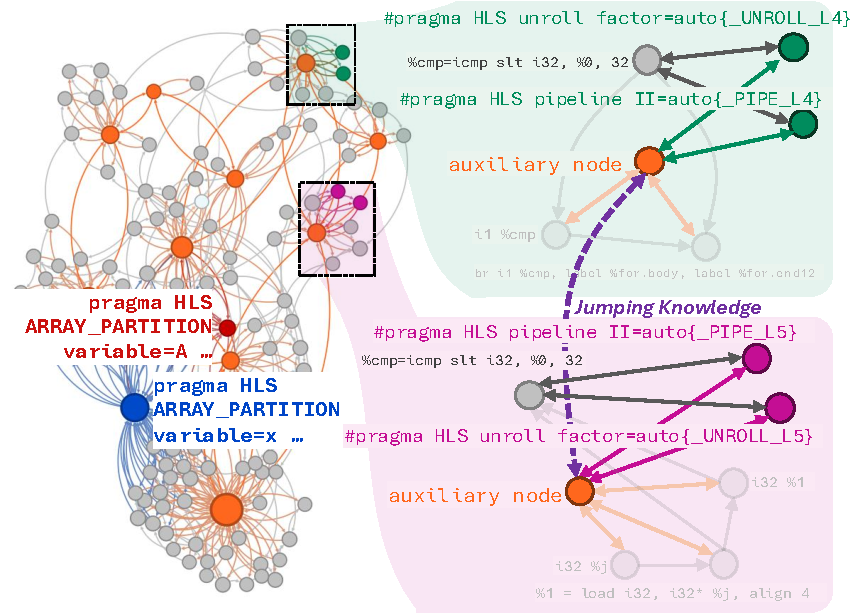
\includegraphics[width=\columnwidth]{figures/02__Methodology/GEMV_Graph-crop.pdf}
    \caption{Structural graph for the GEMV. \figuretodo{\figuretodo{Replace LLVM/icmp nodes with representative Affine/SCF/MemRef operations. Visually distinguish ordinary compiler graph relations from the action-level routing relations consumed by Stage 2. The latter should show self, nearest loop parent/child, array-access scope, and proven dependence forward/reverse.}}}
    \label{fig:gemv-graph}
\end{figure}


A previous version of our work used HARP's hierarchical LLVM graph~\cite{sohrabizadeh2023harp}, we isolate the representation change under a matched GNN control: design points, directive encodings, labels, split, architecture, optimizer, initialization and checkpoint rule are identical; only the graph and native features differ. 

Table~\ref{tab:representation-predictive} reports
graph statistics and selection-relevant ranking metrics. For predictive behavior, Kendall's $\tau_b$ measures how well the surrogate preserves the measured QoR ordering within a target context. Top-1 regret measures the cost of acting on that ranking:
%
\[
R_1=\frac{q(\hat d)}{q(d_{\mathrm{best}})}-1,
\]
%
where $\hat d$ is the design ranked first by the predictor and $d_{\mathrm{best}}$ is the best measured feasible design in the same context. Thus higher $\tau_b$ and lower regret are better.



Both representations align all 544 source actions. Structured MLIR uses 49\% fewer median nodes and 45\% fewer edges while exposing 12 versus 7 relation types; it also improves area/latency $\tau_b$ and reduces top-1 regret by 11.6\%/13.6\%. We therefore adopt it because it is more compact and better aligned with the action-level ranking signal required downstream.

\begin{table}[t]
  \centering
  \caption{\textbf{Matched graph-representation comparison.}
  Structural statistics are median [Q1--Q3] across 55 kernels;
  predictive metrics are macro-averaged across 24 validation
  kernel/device/clock groups (13,011 design points).}
  \label{tab:representation-predictive}

  \scriptsize
  \setlength{\tabcolsep}{3.0pt}
  \renewcommand{\arraystretch}{1.05}

  \begin{tabular}{lrr}
    \toprule
    \textbf{Metric} &
    \textbf{HARP-Rep} &
    \textbf{Structured MLIR} \\
    \midrule

    \multicolumn{3}{l}{\emph{Representation audit}} \\
    Action points aligned
        & 544/544 & 544/544 \\
    Nodes/kernel
        & 645 [361--1008] & 328 [159--542] \\
    Edges/kernel
        & 2,283 [1,269--3,684] & 1,267 [624--2,646] \\
    Relation types/kernel
        & 7 [6--7] & 12 [11--12] \\
    R/M/C/D/U edges
        & 0/0/0/0/0 & 24/66/3/5/12 \\

    \midrule
    \multicolumn{3}{l}{\emph{Selection-relevant prediction}} \\
    Area Kendall $\tau_b$ $\uparrow$
        & 0.284 & \textbf{0.316} \\
    Latency Kendall $\tau_b$ $\uparrow$
        & 0.201 & \textbf{0.224} \\
    Area top-1 regret $\downarrow$
        & 4.232 & \textbf{3.742} \\
    Latency top-1 regret $\downarrow$
        & 0.404 & \textbf{0.349} \\

    \bottomrule
  \end{tabular}

  \vspace{1pt}
  \parbox{0.98\columnwidth}{\scriptsize
  R/M/C/D/U denote region, memory-access, loop-carried,
  proven-dependence, and unresolved-dependence relations.
  A zero indicates that the relation is not encoded as a distinct
  edge class; it does not imply that no related information can be
  inferred transitively from the original graph.}
\end{table}






\subsubsection{QoR-Supervised GNN and Structural Memory}
\label{subsubsec:gnn-backbone}

Each graph is encoded by four edge-aware TransformerConv layers with 64-dimensional states and JK-max aggregation~\cite{xu2018jumping};
graph pooling and latency/resource heads are used only during GNN training. QoR supervision encourages the representation to preserve hardware-relevant dependence, parallelism, and memory information.

At export, prediction heads and directive-value features are removed.
For each $L_k$, we concatenate a 64-D early-layer state, preserving local compiler context, with the 64-D JK state, capturing a wider receptive field. Training-set centering/RMS normalization yields the 128-D pragma-free structural memory used by Stage~2. Device, clock, budget, and objective conditioning remain in the language policy.




\subsection{Target-Conditioned Structural-Semantic Policy}
\label{subsec:llm-backbone}

\framework learns $p(\mathbf d\mid\text{source},o,\tau)$ over the source-derived action points. Stage~1 learns the target/objective-conditioned semantic policy; Stage~2 freezes it and learns gated access to action-aligned compiler memory.


\subsubsection{LLM Prompt Construction}
\label{subsubsec:prompt}

For each action $L_k$, \texttt{<SRC\_Lk>} marks its source location and \texttt{<Lk>} anchors the corresponding output assignments.
Assignment names and order are fixed; the model predicts only directive values, and $L_k$ also serves as the Stage~2 routing identity.
The prompt supplies objective, FPGA, clock, and component-wise BRAM/DSP/FF/LUT budgets as both counts and fractions of device capacity. During Stage~1, the same kernel/device/clock case is presented under multiple budgets, with supervision drawn only from
designs feasible under all four limits.

Among feasible candidates, the objective-specific ranking determines the measured configuration used as supervision; the ranking and budget-sampling policy are detailed in \S\ref{subsec:eval-data}.



\subsubsection{Target-Aware Conditioning}
\label{subsubsec:target-conditioning}

For specified-clock inference, the deployment target is
\[
\tau=(d,c,\mathbf b),\qquad
\mathbf b=(b_{\rm BRAM},b_{\rm DSP},b_{\rm FF},b_{\rm LUT}).
\]
Stage~1 minimizes cross-entropy only at directive value positions, conditioned jointly on source, objective $o$, and $\tau$; fixed anchors and directive syntax are not supervised. Thus identical source code under different clocks or budgets forms different conditional examples: a policy that ignores $\tau$ cannot fit conflicting target-specific assignments. Stage~2 preserves this interface and adds only structural evidence.

% \begin{table}[t]
%     \centering
%     \caption{Target responsiveness of GPT-5.6 Sol, the strongest general-purpose LLM in our evaluation, on GAN. Each row changes only
%     the indicated target attribute relative to C0. Speedup is measured
%     against the pragma-free baseline synthesized for the same device and
%     clock. $\Delta$Dir. denotes the fraction of the 25 directive-value
%     fields changed relative to C0.}
%     \label{tab:gpt_target_responsiveness}
%     \scriptsize
%     \setlength{\tabcolsep}{3.0pt}
%     \renewcommand{\arraystretch}{1.05}
%     \begin{tabular}{lrrrr}
%         \toprule
%         \textbf{Target} &
%         \textbf{Speedup} &
%         \textbf{Res. (\%)} &
%         \textbf{$\Delta$Dir.} &
%         \textbf{Feas.} \\
%         \midrule
%         C0: Latency, ZCU104, 10\,ns
%             & 149.96$\times$ & 26.73 & 0\%  & Yes \\
%         Objective $\rightarrow$ Area
%             &   1.00$\times$ &  1.20 & 60\% & Yes \\
%         Objective $\rightarrow$ ADP
%             & 125.80$\times$ &  6.09 & 20\% & Yes \\
%         Budget $\rightarrow$ 15\%
%             &  78.72$\times$ &  8.45 & 20\% & No$^\dagger$ \\
%         Device $\rightarrow$ U200
%             & 155.13$\times$ &  5.87 & 12\% & Yes \\
%         Clock $\rightarrow$ 3.33\,ns
%             & 172.70$\times$ & 26.63 & 12\% & Yes \\
%         \bottomrule
%     \end{tabular}

%     \vspace{1pt}
%     \parbox{\columnwidth}{\scriptsize
%     $^\dagger$The synthesized design exceeds the requested tight
%     component-wise budget only in LUTs
%     ($1.036\times$ the allowed LUT budget).}
% \end{table}

\begin{figure}[t]
    \centering
    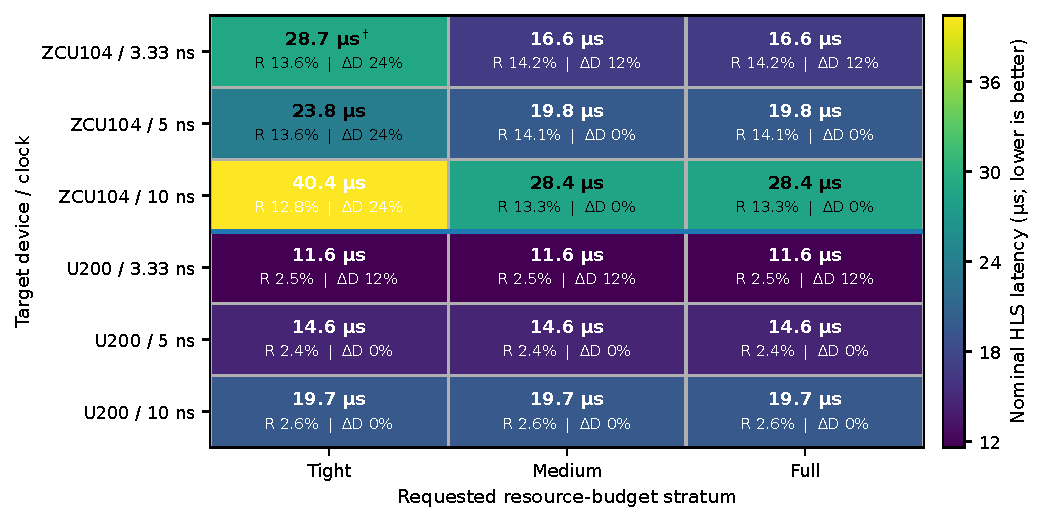
\includegraphics[
        width=0.97\columnwidth
    ]{figures/02__Methodology/target_conditioning_heatmap.pdf}
    \caption{
        \textbf{Target conditioning across device, clock, and resource
        requests on GAN.}
        Each synthesized target reports latency (top), mean resource
        utilization $R$, and the directive change $\Delta D$ relative to
        ZCU104/10\,ns/full. Lower latency is better; $\dagger$ denotes a
        missed requested clock.
    }
    \Description{
        Heatmap of eighteen synthesized SALT-HLS configurations across
        two FPGA devices, three clock periods, and three resource-budget
        strata.
    }
    \label{fig:target-conditioning}
\end{figure}

Figure~\ref{fig:target-conditioning} confirms that these target fields affect the emitted policy. On ZCU104/10\,ns, tightening the budget changes 24\% of directive fields and trades latency (28.4$\rightarrow$40.4\,$\mu$s) for lower resource use; changing clock similarly changes the assignment. Conversely, the three U200 budgets select the same directives when the limits are non-binding, showing that the policy does not change merely because a prompt number changes. The missed 3.33\,ns case also emphasizes that target conditioning does not replace post-generation HLS validation.



\subsubsection{LLM Backbone \& Structural Embeddings Fusion}
\label{subsubsec:structural-fusion}

Stage~2 turns the target-conditioned language policy into an action-grounded structural policy. The decoder hidden state provides the semantic and target-aware query, whereas the action-aligned GNN memory of \S\ref{subsubsec:gnn-backbone} provides compiler-derived keys and values. The Stage~1 policy is frozen: Stage~2 learns only how structural evidence should correct an already functional directive policy.

For a directive RHS position associated with action $L_k$, the structural update can be written schematically as
%
\[
\tilde{\mathbf h}_t =
\mathbf h_t +
\tanh(g)\,
\mathrm{XAttn}(\mathbf h_t,\mathbf M;\mathbf A_k),
\qquad t\in\mathcal R_k .
\]
%
where $\mathbf h_{\mathrm{SA}}$ is the representation after causal self-attention, $\mathbf M$ is the structural-memory bank, $\mathbf A_k$ is the compiler-derived routing mask for $L_k$, and $g$ is a learned residual gate. Structural fusion is therefore selective in two independent ways: only directive-value positions receive the update, and each such position can inspect only structural slots related to its current action.

Cross-attention is applied after the self-attention residual and before the block's feed-forward transformation. This ordering first lets the causal decoder combine source, objective, and target context, then lets that contextualized directive state query compiler memory before further local transformation. The residual gate is initialized at zero, so inserting the structural path initially reproduces the frozen Stage~1 policy and structural corrections are introduced only as training opens the gate.

DeepSeek-Coder-6.7B contains 32 decoder layers; we insert structural fusion after every eighth layer, yielding four interaction points distributed over the backbone. This provides repeated access to compiler evidence without modifying every pretrained block. During Stage~2, the backbone, Stage~1 LoRA, and special-token embeddings remain frozen; only structural cross-attention and its gates are optimized. We evaluate the sensitivity to fusion frequency below and report the remaining architectural hyperparameters in \S\ref{subsec:eval-training}.


\paragraph{Does aligned structural memory matter?}
We test the structural pathway with a fixed-checkpoint intervention rather than retraining separate models. The same frozen ADP policy is evaluated on 18 post-freeze Kalman contexts spanning device, clock, and resource requests. The contexts are selected without QoR information: within each device/clock group we take three evenly spaced quantiles of requested resource fraction. Across interventions we keep the backbone, Stage~1 LoRA, Stage~2 cross-attention weights, decoding rule, and target request identical; only the memory presented to Stage~2 changes.

\emph{Zero} preserves the Stage~2 architecture and routing masks but sets the structural values to zero, testing whether the added fusion machinery alone changes the policy. \emph{Deranged} preserves the same within-kernel set of non-zero structural vectors but applies a deterministic permutation with no action retaining its original vector, breaking the correspondence between $L_k$ and its compiler representation while preserving memory magnitude and cardinality. \emph{Aligned} supplies each $L_k$ with its correct MLIR-derived memory. The comparison therefore separates (i) adding a structural pathway, (ii) supplying arbitrary non-zero side information, and (iii) supplying compiler information under the correct action identity.

Table~\ref{tab:memory-ablation} shows a representative ZCU104/10\,ns synthesis; speedups use the same pragma-free baseline and resource entries are percentages of device capacity in [BRAM, DSP, FF, LUT] order.

\begin{table}[t]
    \centering
    \caption{\textbf{Fixed-checkpoint structural-memory intervention on a
    representative Kalman target} (ZCU104, 10\,ns, full device budget).}
    \label{tab:memory-ablation}
    \scriptsize
    \setlength{\tabcolsep}{3.0pt}
    \renewcommand{\arraystretch}{1.08}

    \begin{tabular}{lccr}
        \toprule
        \textbf{Policy} &
        \textbf{Speedup} &
        \textbf{Feas.} &
        \textbf{[BRAM,DSP,FF,LUT] (\%)} \\
        \midrule
        Stage 1
          & 1.23$\times$  & No  & [183.97,0.12,1.19,8.14] \\
        Stage 2--Zero
          & 1.23$\times$  & No  & [183.97,0.12,1.19,8.14] \\
        Stage 2--Deranged
          & 19.43$\times$ & No  & [183.97,0.23,1.57,8.30] \\
        Stage 2--Aligned
          & \textbf{20.70$\times$} & \textbf{Yes}
          & [96.79,0.23,1.53,8.26] \\
        \bottomrule
    \end{tabular}
\end{table}

The representative synthesis illustrates the three controls clearly.
Zero memory exactly reproduces Stage~1 (1.23$\times$ and 183.97\% BRAM), showing that the additional cross-attention topology alone does not explain the gain. Deranged memory strongly changes the policy and reaches 19.43$\times$ speedup, confirming that the structural branch is active, but it retains the catastrophic 183.97\% BRAM allocation. Restoring the correct action--memory correspondence preserves the acceleration (20.70$\times$) while reducing BRAM to 96.79\%, making the configuration feasible. Thus the useful effect in this case is not simply ``more side
information'': the structural evidence must be associated with the action whose directive is being predicted. 



\paragraph{LLM backbone capacity.}

% \begin{figure}[t]
%     \centering
%     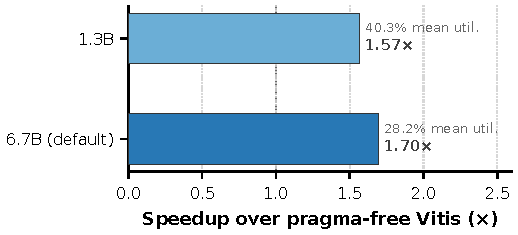
\includegraphics[
%         width=0.96\columnwidth
%     ]{figures/02__Methodology/backbone_capacity_sensitivity.pdf}
%     \caption{
%         \textbf{Backbone-capacity sensitivity on JPEG.}
%         We compare the production 6.7B backbone with a 1.3B variant
%         while retaining the same latency-oriented SALT-HLS task.
%         Labels report measured speedup and mean BRAM/DSP/FF/LUT
%         utilization. The larger backbone improves synthesized QoR while
%         requiring a smaller hardware resource footprint.
%     }
%     \Description{
%         Horizontal bar chart comparing 1.3B and 6.7B SALT-HLS
%         backbones on JPEG by synthesized speedup over pragma-free Vitis.
%         Labels additionally report mean FPGA resource utilization.
%     }
%     \label{fig:backbone-capacity}
% \end{figure}

\EV{small paragraph explaining the backbone capacity experiment, why did we choose this experimental setup (covariance), what conclusions can we draw from it, results with numbers when we insert figure}


\paragraph{Cross-attention placement}

\EV{small paragraph explaining the xattn placement experiment, why did we choose this experimental setup (jpeg), what conclusions can we draw from it, results with numbers when we insert figure}

\EV{Our gains come from SALT architecture rather than the backbone size}


\subsubsection{Objective-Aware Specialization}
\label{subsubsec:peft}

Target conditioning specifies the deployment constraints, whereas the objective selects the preferred feasible trade-off. We therefore share
the code backbone and target interface but maintain separate LoRA adapters~\cite{hu2022lora} for latency, area, and ADP; at inference, $o$ selects the corresponding adapter. This avoids collapsing conflicting objective updates into one policy without duplicating the backbone.


\paragraph{Preference alignment.}
Stage~3 completes the \framework training pipeline by aligning the structurally grounded Stage~2 policy with whole-design hardware preferences.
We construct preference pairs from complete directive configurations evaluated under the same kernel, device, clock, resource budget, and objective; the
chosen design has better measured objective QoR than the rejected one. Holding the target context fixed ensures that the preference signal reflects the directive configuration itself rather than an easier deployment setting. 
We then apply reference-based DPO~\cite{rafailov2023dpo}, which increases the relative likelihood of the preferred complete configuration without training a separate reward model. This whole-design objective complements the token-level supervision of Stages~1--2: it captures interactions among pipeline, unroll, and partition decisions that cannot be attributed reliably to individual directive fields. During Stage~3, the Stage~1 semantic LoRA remains fixed while the structural-fusion parameters are refined, preserving the learned target-conditioned policy while aligning its final decisions with measured hardware preference.



\subsubsection{Automatic Clock Selection}
\label{subsubsec:auto-clock}

If the clock is unspecified, a separate selector chooses $\hat c\in\mathcal C(d)$ from the device-defined measured clock menu using the frozen structural memory and target/objective context.
Training labels select the clock whose best feasible same-context design minimizes the requested objective. \framework then rewrites the request as $(d,\hat c,\mathbf b,o)$ and invokes the ordinary specified-clock policy once. \textsc{Auto} therefore adds one discrete choice rather than an iterative clock--pragma search.\EV{mention the clock accuracy}